\section{Results}
\label{sec:results}

\subsection{TUM RGB-D Validation}

Table~\ref{tab:tum_rgbd_sparse_view} summarizes the 3/5/8/10-view validation run on
\texttt{freiburg1\_room}. The run exercises the complete path from RGB frames to VGGT
geometry, SAM proposals, CLIP+DINOv2 descriptors, object fusion, open-vocabulary
labels, and spatial relations. As the view count increases, lifted proposals increase
from 58 to 198, multi-view object support increases from 18 to 28 nodes, and mean
uncertainty decreases from 0.014525 to 0.011513. This establishes the expected
single-scene behavior before moving to the five-sequence benchmark.

\begin{table}[t]
\centering
\caption{Sparse-view curve on TUM RGB-D \texttt{freiburg1\_room}.}
\label{tab:tum_rgbd_sparse_view}
\small
\resizebox{\linewidth}{!}{%
\begin{tabular}{rrrrrrr}
\toprule
Views & Candidates & Objects & Multi-view & Relations & Uncertainty & MV Ratio \\
\midrule
3 & 58 & 27 & 18 & 466 & 0.014525 & 0.666667 \\
5 & 98 & 32 & 24 & 628 & 0.014585 & 0.750000 \\
8 & 158 & 30 & 26 & 580 & 0.011999 & 0.866667 \\
10 & 198 & 32 & 28 & 636 & 0.011513 & 0.875000 \\
\bottomrule
\end{tabular}
}
\end{table}


\subsection{Component Ablation}

Table~\ref{tab:local_ablation} compares local variants on the development scene. With
the number of lifted candidates fixed, moving from geometry-only OpenCV proposals to
feature-aware fusion lowers mean uncertainty and increases multi-view support. Replacing
OpenCV proposals with SAM masks produces more fused objects and relations, and adding
DINOv2 to CLIP yields the richest graph among the tested variants. This ablation is
local rather than a full benchmark, but it supports the design choice of combining
class-agnostic mask proposals with complementary language-aligned and self-supervised
features.

\begin{table}[t]
\centering
\caption{Development-scene component ablation on a four-view example.}
\label{tab:local_ablation}
\resizebox{\linewidth}{!}{%
\begin{tabular}{lllrrrrr}
\toprule
Variant & Proposals & Features & Candidates & Objects & Multi-view & Relations & Uncertainty \\
\midrule
OpenCV geometry-only & OpenCV & none & 80 & 14 & 9 & 100 & 0.039071 \\
OpenCV feature fusion & OpenCV & clip+handcrafted & 80 & 16 & 10 & 142 & 0.024012 \\
SAM semantic fusion & SAM & clip & 80 & 22 & 15 & 278 & 0.021765 \\
Full pipeline & SAM & clip+dinov2 & 80 & 33 & 17 & 618 & 0.021568 \\
\bottomrule
\end{tabular}
}
\end{table}


\subsection{Benchmark Results}

Table~\ref{tab:tum_rgbd_paper_subset_by_view} reports the five-sequence sparse-view
benchmark. It contains 20 runs: five scenes evaluated at 3, 5, 8, and 10 input views
with the same VGGT, SAM, CLIP+DINOv2, labeling, fusion, and relation inference code.
Averaged over scenes, increasing the view count from 3 to 10 raises lifted object
candidates from 54.0 to 173.6, fused object nodes from 31.8 to 72.2, multi-view object
nodes from 11.8 to 28.2, and inferred spatial relations from 585.2 to 2104.0. The
growth in multi-view nodes is important: additional views do not merely add isolated
proposals, but increase the number of objects supported by evidence from multiple
images. The structural counts measure graph coverage; label and relation consistency
are evaluated separately below.

\begin{table}[t]
\centering
\caption{Average sparse-view scene graph statistics over five TUM RGB-D sequences.}
\label{tab:tum_rgbd_paper_subset_by_view}
\small
\resizebox{\linewidth}{!}{%
\begin{tabular}{rrrrrrr}
\toprule
Views & Scenes & Candidates & Objects & Multi-view & Relations & Uncertainty \\
\midrule
3 & 5 & 54.00 & 31.80 & 11.80 & 585.20 & 0.026421 \\
5 & 5 & 88.60 & 42.80 & 16.80 & 912.80 & 0.035933 \\
8 & 5 & 140.20 & 61.40 & 24.20 & 1472.40 & 0.036613 \\
10 & 5 & 173.60 & 72.20 & 28.20 & 2104.00 & 0.034249 \\
\bottomrule
\end{tabular}
}
\end{table}


Table~\ref{tab:tum_rgbd_paper_subset_results} gives the per-scene breakdown. The full
run outputs are stored under
\texttt{results/benchmark\_tum\_rgbd\_paper\_subset/}; aggregate statistics are exported
to \texttt{sparse\_view\_scene\_graph\_summary.csv} and proxy metrics to
\texttt{sparse\_view\_scene\_graph\_metrics.csv}. Checked reference-consistency
metrics are exported to \texttt{sparse\_view\_checked\_metrics.csv}.

\begin{table}[t]
\centering
\caption{Per-scene sparse-view scene graph statistics on the TUM RGB-D benchmark subset.}
\label{tab:tum_rgbd_paper_subset_results}
\small
\resizebox{\linewidth}{!}{%
\begin{tabular}{lrrrrrr}
\toprule
Scene & Views & Candidates & Objects & Multi-view & Relations & Uncertainty \\
\midrule
freiburg1\_desk & 3 & 56 & 33 & 13 & 602 & 0.032715 \\
freiburg1\_desk & 5 & 93 & 44 & 16 & 752 & 0.031488 \\
freiburg1\_desk & 8 & 153 & 70 & 26 & 1314 & 0.037485 \\
freiburg1\_desk & 10 & 193 & 81 & 30 & 1718 & 0.044303 \\
freiburg1\_desk2 & 3 & 41 & 31 & 5 & 414 & 0.031997 \\
freiburg1\_desk2 & 5 & 66 & 42 & 14 & 694 & 0.040113 \\
freiburg1\_desk2 & 8 & 113 & 79 & 20 & 1602 & 0.042473 \\
freiburg1\_desk2 & 10 & 151 & 110 & 25 & 3564 & 0.038729 \\
freiburg1\_room & 3 & 57 & 41 & 10 & 1088 & 0.022612 \\
freiburg1\_room & 5 & 93 & 64 & 15 & 2100 & 0.024899 \\
freiburg1\_room & 8 & 134 & 76 & 25 & 2836 & 0.022970 \\
freiburg1\_room & 10 & 158 & 80 & 30 & 3192 & 0.021626 \\
freiburg2\_xyz & 3 & 56 & 31 & 14 & 484 & 0.022882 \\
freiburg2\_xyz & 5 & 91 & 33 & 19 & 518 & 0.022266 \\
freiburg2\_xyz & 8 & 144 & 42 & 24 & 840 & 0.025731 \\
freiburg2\_xyz & 10 & 169 & 47 & 26 & 1130 & 0.024507 \\
freiburg3\_long\_office\_household & 3 & 60 & 23 & 17 & 338 & 0.021901 \\
freiburg3\_long\_office\_household & 5 & 100 & 31 & 20 & 500 & 0.060900 \\
freiburg3\_long\_office\_household & 8 & 157 & 40 & 26 & 770 & 0.054405 \\
freiburg3\_long\_office\_household & 10 & 197 & 43 & 30 & 916 & 0.042079 \\
\bottomrule
\end{tabular}
}
\end{table}


\begin{figure}[t]
\centering
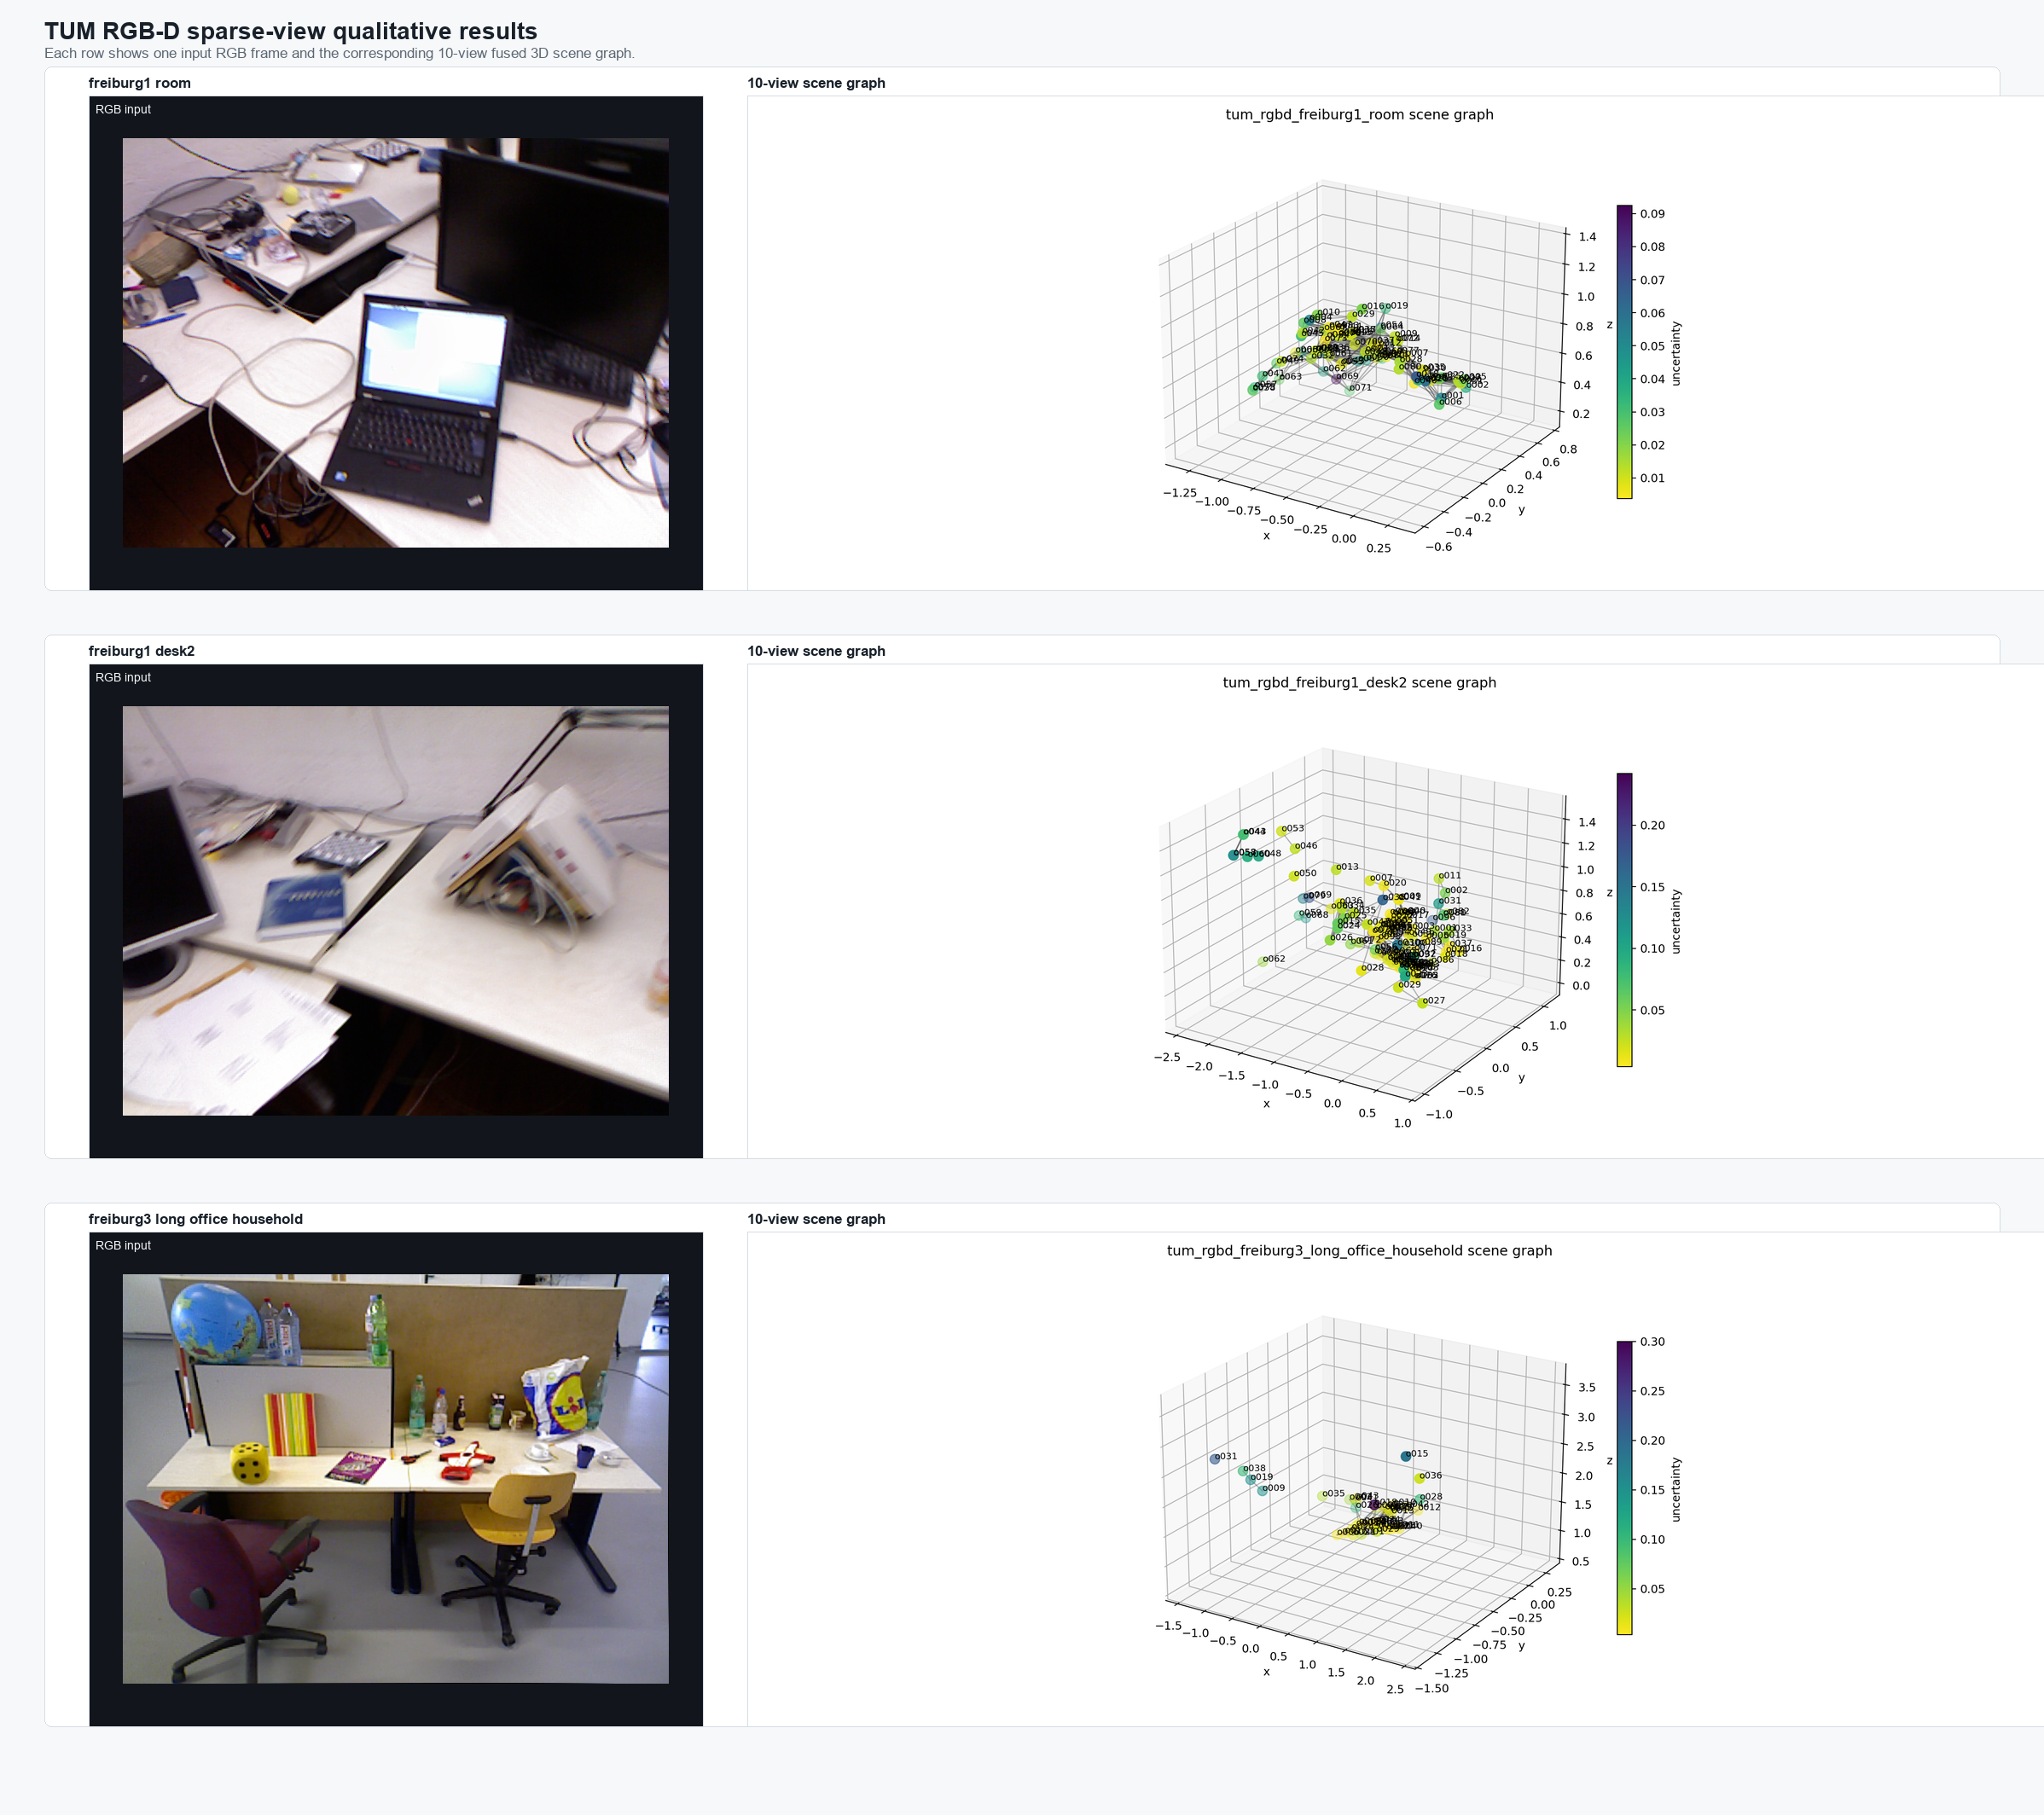
\includegraphics[width=0.98\textwidth]{figures/tum_rgbd_paper_subset_qualitative}
\caption{Qualitative examples from the TUM RGB-D benchmark subset. Each row shows one
input RGB frame and the corresponding 10-view fused 3D scene graph visualization. Node
colors encode uncertainty and edge overlays show inferred near relations.}
\label{fig:tum_rgbd_paper_subset_qualitative}
\end{figure}

Figure~\ref{fig:tum_rgbd_paper_subset_qualitative} shows representative qualitative
outputs from the benchmark. The examples show sparse RGB observations converted into
fused 3D object nodes, uncertainty-colored graph visualizations, and relation overlays.
They also illustrate why uncertainty is retained in the exported graph: sparse-view
nodes and edges can remain ambiguous even when the overall graph is coherent, and the
uncertainty field provides a practical signal for review.

\subsection{Checked Reference-Consistency Metrics}

For the five-scene benchmark, each 10-view graph is converted into a
prediction-seeded annotation draft and checked through the review CSV/JSON path. We
compare the 3/5/8-view outputs against those checked reference sets and include the
10-view row as a reference construction check.
Table~\ref{tab:tum_rgbd_paper_subset_checked_by_view} summarizes the five-scene
average. Object-label F1 improves from 0.622 at 3 views to 0.751 at 5 views and 0.914
at 8 views. Labeled relation-triplet F1 improves from 0.434 to 0.561 and 0.799 over
the same view counts. Precision is high even at 3 views, while recall rises
substantially with more views; the main sparse-view failure mode is therefore missing
objects and relation triplets rather than producing many inconsistent labels.

\input{tables/tum_rgbd_paper_subset_checked_by_view}

Table~\ref{tab:tum_rgbd_paper_subset_checked_results} gives the per-scene consistency
scores. The hardest case is \texttt{freiburg1\_desk2}, where relation-triplet F1 is
0.206 at 3 views and 0.616 at 8 views, reflecting the difficulty of recovering a dense
relation set from sparse inputs. The strongest 8-view relation score is on
\texttt{freiburg1\_room} at 0.929, which is also the scene used during development.
This spread shows that the aggregate trend is not caused by one sequence while keeping
the failure modes visible.

\begin{table}[t]
\centering
\caption{Per-scene consistency results against checked prediction-seeded references. The 10-view rows check reference construction rather than independent accuracy.}
\label{tab:tum_rgbd_paper_subset_checked_results}
\small
\resizebox{\linewidth}{!}{%
\begin{tabular}{lrrrrrrr}
\toprule
Scene & Views & Obj P & Obj R & Obj F1 & Rel P & Rel R & Rel F1 \\
\midrule
freiburg1\_desk & 3 & 1.000 & 0.407 & 0.579 & 0.987 & 0.346 & 0.512 \\
freiburg1\_desk & 5 & 1.000 & 0.543 & 0.704 & 0.992 & 0.434 & 0.604 \\
freiburg1\_desk & 8 & 0.971 & 0.840 & 0.901 & 0.962 & 0.736 & 0.834 \\
freiburg1\_desk & 10 & 1.000 & 1.000 & 1.000 & 1.000 & 1.000 & 1.000 \\
freiburg1\_desk2 & 3 & 1.000 & 0.282 & 0.440 & 0.990 & 0.115 & 0.206 \\
freiburg1\_desk2 & 5 & 1.000 & 0.382 & 0.553 & 0.954 & 0.186 & 0.311 \\
freiburg1\_desk2 & 8 & 1.000 & 0.718 & 0.836 & 0.993 & 0.446 & 0.616 \\
freiburg1\_desk2 & 10 & 1.000 & 1.000 & 1.000 & 1.000 & 1.000 & 1.000 \\
freiburg1\_room & 3 & 0.976 & 0.500 & 0.661 & 0.961 & 0.328 & 0.489 \\
freiburg1\_room & 5 & 1.000 & 0.800 & 0.889 & 0.986 & 0.648 & 0.782 \\
freiburg1\_room & 8 & 1.000 & 0.950 & 0.974 & 0.987 & 0.877 & 0.929 \\
freiburg1\_room & 10 & 1.000 & 1.000 & 1.000 & 1.000 & 1.000 & 1.000 \\
freiburg2\_xyz & 3 & 1.000 & 0.660 & 0.795 & 0.955 & 0.409 & 0.572 \\
freiburg2\_xyz & 5 & 1.000 & 0.702 & 0.825 & 0.903 & 0.414 & 0.568 \\
freiburg2\_xyz & 8 & 1.000 & 0.894 & 0.944 & 0.971 & 0.722 & 0.828 \\
freiburg2\_xyz & 10 & 1.000 & 1.000 & 1.000 & 1.000 & 1.000 & 1.000 \\
freiburg3\_long\_office\_household & 3 & 0.913 & 0.488 & 0.636 & 0.722 & 0.266 & 0.389 \\
freiburg3\_long\_office\_household & 5 & 0.935 & 0.674 & 0.784 & 0.764 & 0.417 & 0.540 \\
freiburg3\_long\_office\_household & 8 & 0.950 & 0.884 & 0.916 & 0.862 & 0.725 & 0.788 \\
freiburg3\_long\_office\_household & 10 & 1.000 & 1.000 & 1.000 & 1.000 & 1.000 & 1.000 \\
\bottomrule
\end{tabular}
}
\end{table}

